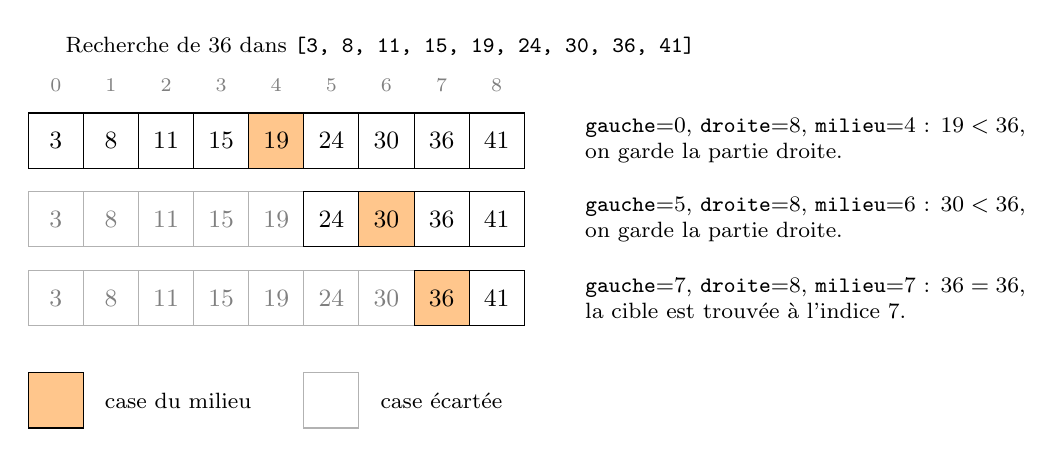
\begin{tikzpicture}[x=1cm,y=1cm,c/.style={draw,minimum size=0.7cm,inner sep=0pt,font=\small},
 mn/.style={fill=orange!45},ok/.style={fill=gray!30},cl/.style={fill=cyan!30},ix/.style={thick,draw=black,line width=1.2pt},hors/.style={text=gray,draw=gray!60},lab/.style={anchor=west,font=\footnotesize,align=left}]
\node[lab] at (0,0.6){Recherche de $36$ dans \texttt{[3, 8, 11, 15, 19, 24, 30, 36, 41]}};
\node[font=\scriptsize,gray] at (0.00,0.1){0};
\node[font=\scriptsize,gray] at (0.70,0.1){1};
\node[font=\scriptsize,gray] at (1.40,0.1){2};
\node[font=\scriptsize,gray] at (2.10,0.1){3};
\node[font=\scriptsize,gray] at (2.80,0.1){4};
\node[font=\scriptsize,gray] at (3.50,0.1){5};
\node[font=\scriptsize,gray] at (4.20,0.1){6};
\node[font=\scriptsize,gray] at (4.90,0.1){7};
\node[font=\scriptsize,gray] at (5.60,0.1){8};
\node[c,] at (0.00,-0.60) {3};
\node[c,] at (0.70,-0.60) {8};
\node[c,] at (1.40,-0.60) {11};
\node[c,] at (2.10,-0.60) {15};
\node[c,mn] at (2.80,-0.60) {19};
\node[c,] at (3.50,-0.60) {24};
\node[c,] at (4.20,-0.60) {30};
\node[c,] at (4.90,-0.60) {36};
\node[c,] at (5.60,-0.60) {41};
\node[lab] at (6.6,-0.60){\texttt{gauche}=0, \texttt{droite}=8, \texttt{milieu}=4 : $19<36$,\\on garde la partie droite.};
\node[c,hors] at (0.00,-1.60) {3};
\node[c,hors] at (0.70,-1.60) {8};
\node[c,hors] at (1.40,-1.60) {11};
\node[c,hors] at (2.10,-1.60) {15};
\node[c,hors] at (2.80,-1.60) {19};
\node[c,] at (3.50,-1.60) {24};
\node[c,mn] at (4.20,-1.60) {30};
\node[c,] at (4.90,-1.60) {36};
\node[c,] at (5.60,-1.60) {41};
\node[lab] at (6.6,-1.60){\texttt{gauche}=5, \texttt{droite}=8, \texttt{milieu}=6 : $30<36$,\\on garde la partie droite.};
\node[c,hors] at (0.00,-2.60) {3};
\node[c,hors] at (0.70,-2.60) {8};
\node[c,hors] at (1.40,-2.60) {11};
\node[c,hors] at (2.10,-2.60) {15};
\node[c,hors] at (2.80,-2.60) {19};
\node[c,hors] at (3.50,-2.60) {24};
\node[c,hors] at (4.20,-2.60) {30};
\node[c,mn] at (4.90,-2.60) {36};
\node[c,] at (5.60,-2.60) {41};
\node[lab] at (6.6,-2.60){\texttt{gauche}=7, \texttt{droite}=8, \texttt{milieu}=7 : $36=36$,\\la cible est trouvée à l'indice 7.};
\node[c,mn] at (0,-3.9){};\node[lab] at (0.5,-3.9){case du milieu};\node[c,hors] at (3.5,-3.9){};\node[lab] at (4.0,-3.9){case écartée};
\end{tikzpicture}